% !TeX program = pdflatex
% =============================================================
% Public Economics -- Lecture 1
% Why Study Public Finance?
% Based on: Gruber, J. "Public Finance and Public Policy", Ch. 1
% Austrian institutional and empirical context added for WU Vienna.
% =============================================================
\documentclass[11pt,aspectratio=169]{beamer}

\usetheme{metropolis}
\usepackage[utf8]{inputenc}
\usepackage[T1]{fontenc}
\usepackage{lmodern}
\usepackage{booktabs}
\usepackage{array}
\usepackage{textcomp}
\usepackage{siunitx}
\usepackage{tikz}
\usepackage{pgfplots}
\pgfplotsset{compat=1.18}
\usepackage{pgf-pie}
\usetikzlibrary{positioning,arrows.meta,calc}

% ----------------------------------------------------------------
% Colors: WU Vienna blue as primary accent
% ----------------------------------------------------------------
\definecolor{wublue}{HTML}{003D7C}
\definecolor{wulight}{HTML}{4F8FC4}
\definecolor{wugray}{HTML}{5C6670}
\definecolor{wured}{HTML}{B0202E}
\definecolor{wugreen}{HTML}{4C8C6B}
\definecolor{wuyellow}{HTML}{D9A441}
\setbeamercolor{palette primary}{bg=wublue,fg=white}
\setbeamercolor{frametitle}{bg=wublue,fg=white}
\setbeamercolor{progress bar}{fg=wublue,bg=wulight!30}
\setbeamercolor{alerted text}{fg=wured}

\setbeamertemplate{frame footer}{Why Study Public Economics?}
\setbeamertemplate{footline}[frame number]

\title{Public Economics}
\subtitle{Lecture 1 \(\cdot\) Why Study Public Economics?}
\author{Dr. Shushanik Margaryan}
\institute{WU Vienna University of Economics and Business}
\date{Winter Term}

% Source note command for footnote-style citations on data slides
\newcommand{\srcnote}[1]{{\footnotesize\color{wugray}Source: #1}}

\begin{document}

% =============================================================
\begin{frame}
  \titlepage
\end{frame}

\begin{frame}
	\frametitle{Nuts and bolts}

	\begin{itemize}
		\item This course provides a foundational introduction to public economics
		\item We meet on Tuesdays from 2pm-6pm
		\item There will be a break from 3:45-4:15
		\item Attendance is compulsory. A max of 2 missed sessions is permitted
	\end{itemize}

	\begin{figure}
		\centering
		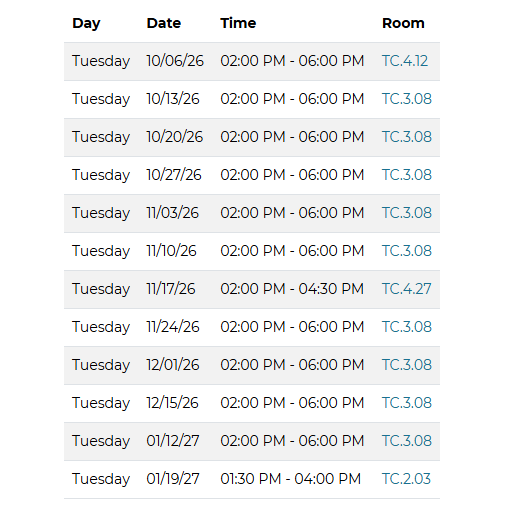
\includegraphics[scale=0.36]{schedule}

	\end{figure}

\end{frame}

\begin{frame}
	\frametitle{Assessment}
\begin{itemize}
			\item A maximum of 100 points can  be achieved in total.
	\begin{itemize}

		\item 3 homework assignments: 3 × 6 points= 18
		\item A midterm and an endterm exam, each worth of 30 points
		\item Report (1–3 pages) on a selected research paper in Focus Area 2 = 12 points.

	\end{itemize}

	\item A min of one point needs to be achieved in each subtask to receive a passing grade.

	\item Grading scale:

	$<$ 60 points:             Unsatisfactory;
	60 points or above: Sufficient;
	70 points or above: Satisfactory;
	80 points or above: Good;
	90 points or above: Excellent;



\end{itemize}
\end{frame}



	\begin{frame}{Paper Report: Formal Criteria}
		\begin{itemize}
			\item PDF document; your name in the file name \emph{and} the header!
			\item 1--3 pages; more pages does not mean a better score
			\item English or German
			\item Inclusive language
			\item Coherent phrasing, a clear thread throughout, correct spelling, proper citation
			\item No cover page, no table of contents, \ldots
		\end{itemize}
	\end{frame}

	\begin{frame}{Submission}
		\begin{itemize}
			\item Submit via Canvas --- once submitted, it is final
			\item \alert{Submissions are checked for plagiarism!} If the text fails this check, you receive 0 points, and the assessment \emph{cannot} be repeated!
			\item Even translating sentences from the paper into another language counts as plagiarism!
		\end{itemize}
	\end{frame}

	\begin{frame}{Content Structure}
		\begin{itemize}
			\item \textbf{Part 1}: Summary of the paper:A clear and correct description of what the paper is about, Research question, objectives, methods, results,... (max. 1 page!)

			\item \textbf{Part 2}: Discuss which aspect of the paper was most interesting to you. What was particularly well done in the paper? Why are you convinced of this?

			\item \textbf{Part 3}: What is missing in the paper? Describe what you think is underdeveloped in the paper, why this aspect would be important, and how you would improve/supplement it. Stick to the context of the present paper and its objective; do not pose a new research question! Refer to the course content and previous texts.
		\end{itemize}

	\end{frame}

	\begin{frame}{Working Independently}
		\begin{itemize}
			\item Work as independently as possible: formulate results, methodology, and the research question in your \emph{own} words!
			\item Dare to question and critique the papers --- we want you to engage with them critically and independently.
		\end{itemize}
		\begin{alertblock}{A critical use of AI is ok, but}
			\begin{itemize}
				\item AI-based tools analyze complex studies only inadequately.
				\item We discuss the papers in class --- you benefit most if you've already read them yourself.
				\item The papers are  exam-relevant, so doing it yourself saves you time in the end.
			\end{itemize}
		\end{alertblock}
	\end{frame}




\section{Introduction}
% =============================================================
\begin{frame}{Introduction}
  \begin{itemize}
    \item What is \alert{public economics}, and what are the key questions the field addresses?
    \item What are the key facts about the size and growth of government, and the distribution of taxes and spending?
    \item How do the questions of public economics/fiance show up in a concrete policy debate?  
  \end{itemize}
  \vspace{1em}

\end{frame}

% =============================================================
 

% =============================================================
 
% =============================================================
\section{1.1 The Four Questions of Public Economics}

\begin{frame}{What Is Public Economics?}
  \begin{block}{Public Economics}
    The study of the role of \textbf{government} in the economy.
  \end{block}
  \vspace{1em}
  \textbf{The four questions of Public Economics:}
  \begin{enumerate}
    \item \textbf{When} should the government intervene in the economy?
    \item \textbf{How} might the government intervene?
    \item \textbf{What is the effect} of those interventions on economic outcomes?
    \item \textbf{Why} do governments choose to intervene in the way that they do?
  \end{enumerate}
\end{frame}

\begin{frame}{Q1: When Should the Government Intervene?}
  \textbf{Baseline:} in a competitive market, the equilibrium (supply = demand) maximizes the \emph{social efficiency} of trade.
  \begin{itemize}
    \item Every trade valued by both sides happens; no valuable trade is missed.
    \item So the free market is the benchmark --- government intervention needs a \emph{justification}.
  \end{itemize}
  \vspace{1em}
  \begin{alertblock}{Two justifications for intervention}
    \begin{enumerate}
      \item \textbf{Market failure} --- the market outcome is not efficient
      \item \textbf{Redistribution} --- society wants a different \emph{distribution} of the outcome (even if it is efficient)
    \end{enumerate}
  \end{alertblock}
\end{frame}

\begin{frame}{Market Failure}

\textbf{Market failure occurs when a free market fails to allocate resources efficiently.}

\begin{itemize}
	\item Examples of market failures?
\end{itemize}
 \pause
  \begin{itemize}
    \item Health insurance \emph{looks} like a textbook competitive market: many buyers, many sellers.
    \item But: if I skip a flu shot, I raise \emph{my} risk of getting the flu --- and the risk that I infect \emph{you}.
    \item I only weigh \emph{my own} costs and benefits when deciding whether to insure/vaccinate; I ignore the cost I impose on others.
    \item The same logic applies to vaccination generally: below some coverage threshold, \emph{herd immunity} breaks down and outbreaks become possible again --- private vaccination choices under-provide protection relative to the social optimum.
  \end{itemize}
  \vspace{0.5em}
  \centering
  $\Rightarrow$ a \textbf{negative externality}: private decisions $\neq$ socially efficient decisions.
\end{frame}



\begin{frame}{Redistribution}

\textbf{The shifting of resources from some groups in society to others.}

  \begin{itemize}
    \item Think of the economy as a \textbf{pie}: efficiency determines its \emph{size}.
    \item Redistribution reshuffles different groups' shares of the pie
    \item Why? Society may  value \texteuro{}1 more to a poor household than to a rich one.
  \end{itemize}
  \vspace{0.5em}
  \begin{alertblock}{The equity--efficiency trade-off}
  \vspace{0.2cm}
    Redistributive policies can change economic agents' behavior (e.g., work incentives), which can \emph{shrink the pie}
  \end{alertblock}
\end{frame}



\begin{frame}{Q2: How Might the Government Intervene?}
  Four broad policy tools:
  \begin{enumerate}
    \item \textbf{Tax or subsidize}
    \item \textbf{Restrict or mandate}
    \item \textbf{Public provision} (the government produces the good itself)
    \item \textbf{Public financing of private provision} (government pays; private firms produce)
  \end{enumerate}
\end{frame}

\begin{frame}{The Four Tools, With Austrian Examples}
  \begin{center}
  \small
  \begin{tabular}{@{}p{3.4cm}p{8.5cm}@{}}
    \toprule
    \textbf{Tool} & \textbf{Austrian example} \\
    \midrule
    Tax/subsidize & \emph{Pendlerpauschale} (commuter tax deduction); CO\textsubscript{2} pricing under the eco-social tax reform \\[0.4em]
    Mandate/restrict & Covid-19 vaccination mandate (2022, repealed 2023) \\[0.4em]
    Public provision & ÖGK public health insurance; public hospitals (Gemeindespital network) \\[0.4em]
    Public financing of private provision & Social-insurance reimbursement of private physicians and private hospitals \\
    \bottomrule
  \end{tabular}
  \end{center}
\end{frame}

\begin{frame}{Q3: What Are the Effects of Interventions?}
  \begin{block}{Direct effects}
    What would happen \emph{if people did not change their behavior}.
  \end{block}
  \begin{block}{Indirect effects}
    What happens \emph{because} people change their behavior in response.
  \end{block}
  \vspace{1em}
  \centering
  Both matter for evaluating \emph{any} government intervention
\end{frame}





\begin{frame}{Q4: Normative vs.\ Positive Public Economics}
  \begin{block}{Normative}

    Analysis of how things \emph{should} be. \\
    \emph{Should} the government have mandated Covid-19 vaccination? \emph{How high} should the top income tax rate be?
  \end{block}
  \begin{block}{Positive}

    Analysis of how things \emph{really are}. \\
    \emph{Did} the Impfpflicht actually raise vaccination rates? \emph{Does} Kurzarbeit actually prevent layoffs, or mostly subsidize jobs that would have survived anyway?
  \end{block}
  \vspace{0.5em}
  \centering
  \alert{Positive analysis (mostly empirical) is the necessary first step before normative analysis (mostly theoretical) can be completed.}
\end{frame}

% =============================================================
\section{1.2 Facts on Government in Austria}

\begin{frame}{Why Look at the Facts?}
  \begin{itemize}
    \item Public Economics is compelling because government is \emph{everywhere} in economic life.
    \item We now look at some facts about Austria: size, decentralization, deficits/debt, spending composition, revenue composition, etc.
 

  \end{itemize}
\end{frame}

\begin{frame}{A Methodological Note: What Counts as ``Government''?}
  \footnotesize
  Measuring the ``size of government'' first requires deciding \emph{what belongs to} the state sector.
  \begin{itemize}
    \item Under the European System of Accounts (ESVG 2010), Austria's \textbf{Staatssektor} (S.13) comprises \textbf{4{,}973} institutional units across four subsectors: Bund (410), Länder (357), Gemeinden (4{,}156), and Sozialversicherungsträger (50).
    \item Classification depends on \emph{function and market/non-market status}, not ownership: a state-owned firm covering most of its costs from market sales (e.g.\ ÖBB-Personenverkehr, ORF) can fall \emph{outside} the state sector, while a nominally private, state-controlled nonprofit can fall \emph{inside} it.
    \item \textbf{General (``unechte'') Staatsquoten} --- like spending/GDP, on the next slide --- compare a numerator that is \emph{not} a subset of the denominator, which can overstate government's real economic weight.
    \item \textbf{Specific (``echte'') Staatsquoten} compare one budget line to the whole budget (e.g.\ health's share of total spending) and are more directly interpretable.
  \end{itemize}
 
\end{frame}

\begin{frame}{ The Size of Government Has Grown --- Everywhere}
  \begin{itemize}
    \item Government spending has expanded across Western Europe since 1960, driven above all by the build-out of the welfare state.
    \item The pace has varied enormously: Greece's government share roughly tripled since 1960; Sweden's peaked near two-thirds of GDP in the early 1990s before falling back.
    \item Austria's own \textbf{Staatsquote} sits well above the OECD average today (next slide).
  \end{itemize}
  \begin{block}{Discussion}
    What explains the twentieth-century growth of government spending across almost every developed country?
  \end{block}

\end{frame}

\begin{frame}{Government Spending Across the EU --- and the US}
  \begin{center}
  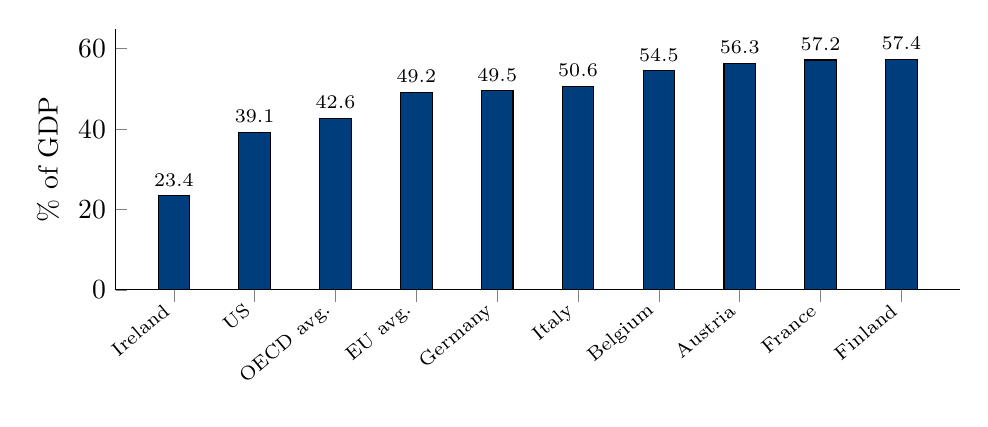
\begin{tikzpicture}
    \begin{axis}[
      ybar, bar width=0.4cm,
      width=12.3cm, height=4.9cm,
      ymin=0, ymax=65,
      symbolic x coords={Ireland,US,OECD avg.,EU avg.,Germany,Italy,Belgium,Austria,France,Finland},
      xtick=data,
      x tick label style={font=\scriptsize, rotate=40, anchor=east},
      ylabel={\% of GDP},
      nodes near coords,
      nodes near coords style={font=\scriptsize},
      enlarge x limits=0.08,
      axis lines*=left,
      every node near coord/.append style={
        /pgf/number format/.cd, fixed, precision=1
      },
      ]
      \addplot[fill=wublue] coordinates {
        (Ireland,23.4) (US,39.1) (OECD avg.,42.6) (EU avg.,49.2) (Germany,49.5)
        (Italy,50.6) (Belgium,54.5) (Austria,56.3) (France,57.2) (Finland,57.4)
      };
    \end{axis}
  \end{tikzpicture}
  \end{center}

\end{frame}

\begin{frame}{Explanatory Approaches to the Growth of Government Spending (1)}
	
	No monocausal, self-contained explanatory approach exists.
	\vspace{0.4em}
	\begin{itemize}
		\item \textbf{Change in the function of state activity}
		\begin{itemize}
			\item Transition from the ``regulatory'' (``night-watchman'') state to the \emph{service-providing} state (\emph{Leistungsstaat}).
			\item The ``law'' of growing state activity / the growing expansion of financing needs; \textbf{Wagner's Law}: growth of ``legal and power purposes'' as well as (expenditure-intensive) ``cultural and welfare purposes''.
			\item Modern (welfare) states assign the state distinctly more, and also new, tasks 
			\item \textbf{Theory of occasional displacements} (Peacock \& Wiseman): the level-displacement effect; tax resistance is overcome in crisis periods, with a ``habituation effect'' carrying the new level into normal times.
		\end{itemize}
	\end{itemize}

\end{frame}

\begin{frame}{Explanatory Approaches to the Growth of Government Spending (2)}

	\begin{itemize}
		\item \textbf{Income elasticity of demand for public services}
		\begin{itemize}
			\item Steadily rising private income / standard of living leads to the expansion of government spending,
			\item because the income elasticity of demand for public services is higher than that for private services.
			\item Assumes that ``higher'' needs are covered to a greater extent by state providers (Maslow's hierarchy of needs).
		\end{itemize}
		\item \textbf{Influence of population density}
		\begin{itemize}
			\item \textbf{Brecht's Law}: the ``law of progressive parallelism between expenditure and population concentration'' links the degree of agglomeration to the level of the government share.
			\item Larger municipalities carry more public tasks (the ``zoo effect'') and often more complex, more expenditure-intensive ones (e.g.\ public transit).
		\end{itemize}
	\end{itemize}

\end{frame}

\begin{frame}{Explanatory Approaches to the Growth of Government Spending (3)}

	\begin{itemize}
		\item \textbf{Low productivity of public services}
		\begin{itemize}
			\item \textbf{Baumol's cost disease} (excessive cost increase) in the public-service sector, resulting from the productivity gap between the goods sector and the service sector, combined with wage solidarity across the public and private sectors.
		\end{itemize}
		\item \textbf{Political-economy explanatory approaches} (public-choice approaches)
		\begin{itemize}
			\item The political process itself as a reason for rising government-spending ratios.
			\item The self-interest of political actors determines the supply of public services.

			\textbf{Rent-seeking} describes the effort of interest groups to influence legislation (``distributional coalitions'') in order to secure special advantages for their members --- politically obtained privileges --- that produce permanent, unearned income in the market sphere.
			\end{itemize}

	\end{itemize}

\end{frame}



\begin{frame}{Decentralization --- Who Spends, Who Taxes?}
  \vspace{1em}
  \begin{alertblock}{Austria's federalism: Expenditure by level of government (2024}
  	\begin{itemize}
  		\item 	Bund \textbf{48\%} (\texteuro{}176.1bn)
  		\item   Sozialversicherung \textbf{25\%} (\texteuro{}93.7bn)
  		\item   Länder \textbf{14\%} (\texteuro{}52.2bn, excl.\ Wien)
  		\item  Gemeinden \textbf{13\%} (\texteuro{}46.7bn, incl.\ Wien)
  	\end{itemize}
 
 
  \end{alertblock}
 

\end{frame}

 

\begin{frame}{Why So Centralized? A Political-Economy View}
  \begin{itemize}
    \item Redistribution is hard to sustain at the local level: if a \emph{Land} or \emph{Gemeinde} taxes high earners heavily on its own, they can simply move to a lower-tax neighbor.
    \item Centralizing revenue at the \textbf{Bund} is what makes Austria's \emph{Finanzausgleich} possible --- transferring resources from richer to poorer regions in a way a fully decentralized system could not.

  \end{itemize}


\end{frame}

\begin{frame}{Deficits and Debt}
  \begin{block}{Definitions}
    \textbf{Deficit} = spending $-$ revenue in a given year.

       \textbf{Debt} = accumulated past deficits.
  \end{block}
  \begin{itemize}
    \item The EU's \textbf{Maastricht rules} cap the deficit at 3\% of GDP and gross debt at 60\% of GDP for member states.

  \end{itemize}

\end{frame}

\begin{frame}{Austria vs.\ the Maastricht Rules (2025)}
  \begin{center}
  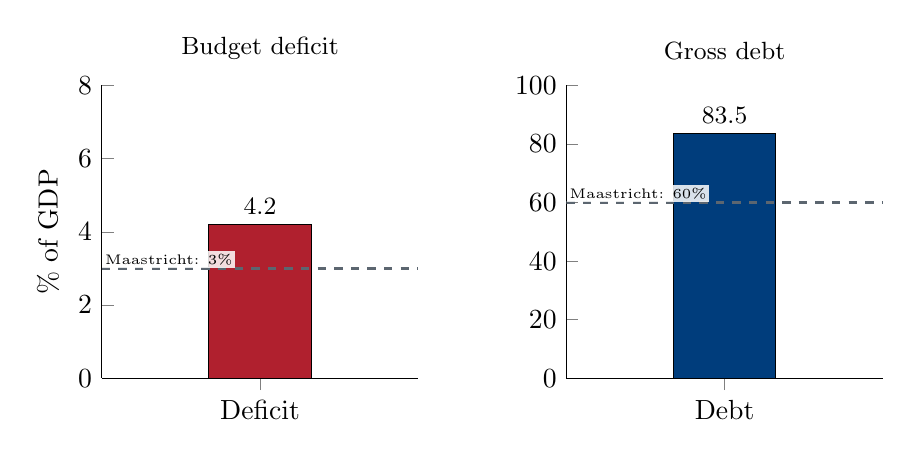
\begin{tikzpicture}
    \begin{axis}[
      ybar, bar width=1.3cm,
      width=5.6cm, height=5.3cm,
      ymin=0, ymax=8,
      symbolic x coords={Deficit},
      xtick=data,
      ylabel={\% of GDP},
      title={Budget deficit},
      title style={font=\small},
      nodes near coords,
      nodes near coords style={font=\small},
      enlarge x limits=1.3,
      axis lines*=left,
      ]
      \addplot[fill=wured] coordinates {(Deficit,4.2)};
      \draw[dashed, thick, wugray] (rel axis cs:0,0.375) -- (rel axis cs:1,0.375);
      \node[anchor=south west, font=\tiny, fill=white, fill opacity=0.85, text opacity=1, inner sep=1pt]
        at (rel axis cs:0,0.375) {Maastricht: 3\%};
    \end{axis}
    \begin{axis}[
      at={($(5.9cm,0)$)},
      ybar, bar width=1.3cm,
      width=5.6cm, height=5.3cm,
      ymin=0, ymax=100,
      symbolic x coords={Debt},
      xtick=data,
      title={Gross debt},
      title style={font=\small},
      nodes near coords,
      nodes near coords style={font=\small},
      enlarge x limits=1.3,
      axis lines*=left,
      ]
      \addplot[fill=wublue] coordinates {(Debt,83.5)};
      \draw[dashed, thick, wugray] (rel axis cs:0,0.6) -- (rel axis cs:1,0.6);
      \node[anchor=south west, font=\tiny, fill=white, fill opacity=0.85, text opacity=1, inner sep=1pt]
        at (rel axis cs:0,0.6) {Maastricht: 60\%};
    \end{axis}
  \end{tikzpicture}
  \end{center}
  \centering \small
  \srcnote{Statistik Austria}
\end{frame}

\begin{frame}{Austria's Revenues and Expenditures Over Time}
  \begin{figure}
  	\centering
  	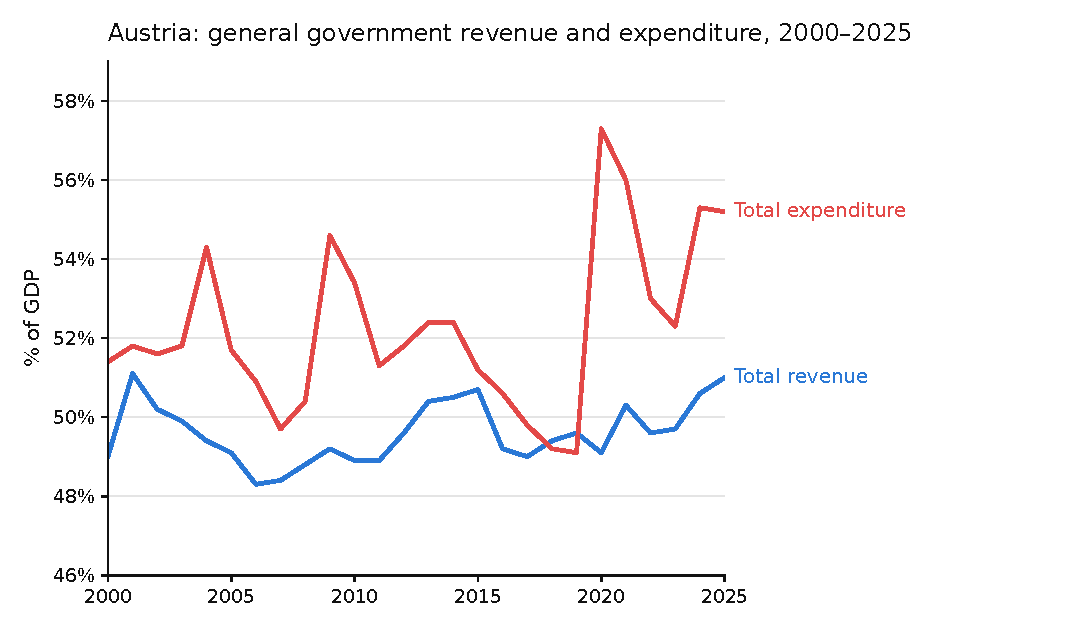
\includegraphics[width=0.7\linewidth]{01_revenue_vs_expenditure}
  \end{figure}
\end{frame}



\begin{frame}{Discussion: Deficits and Debt}
  \begin{itemize}
    \item What are the costs of running larger deficits and carrying more debt?
    \item Why might it make sense to let deficits rise in \emph{some} years (recessions, pandemics) even under fixed fiscal rules?

  \end{itemize}
\end{frame}


\begin{frame}{Austria's Government Expenditure, by Function}
   \begin{figure}
 	\centering
 	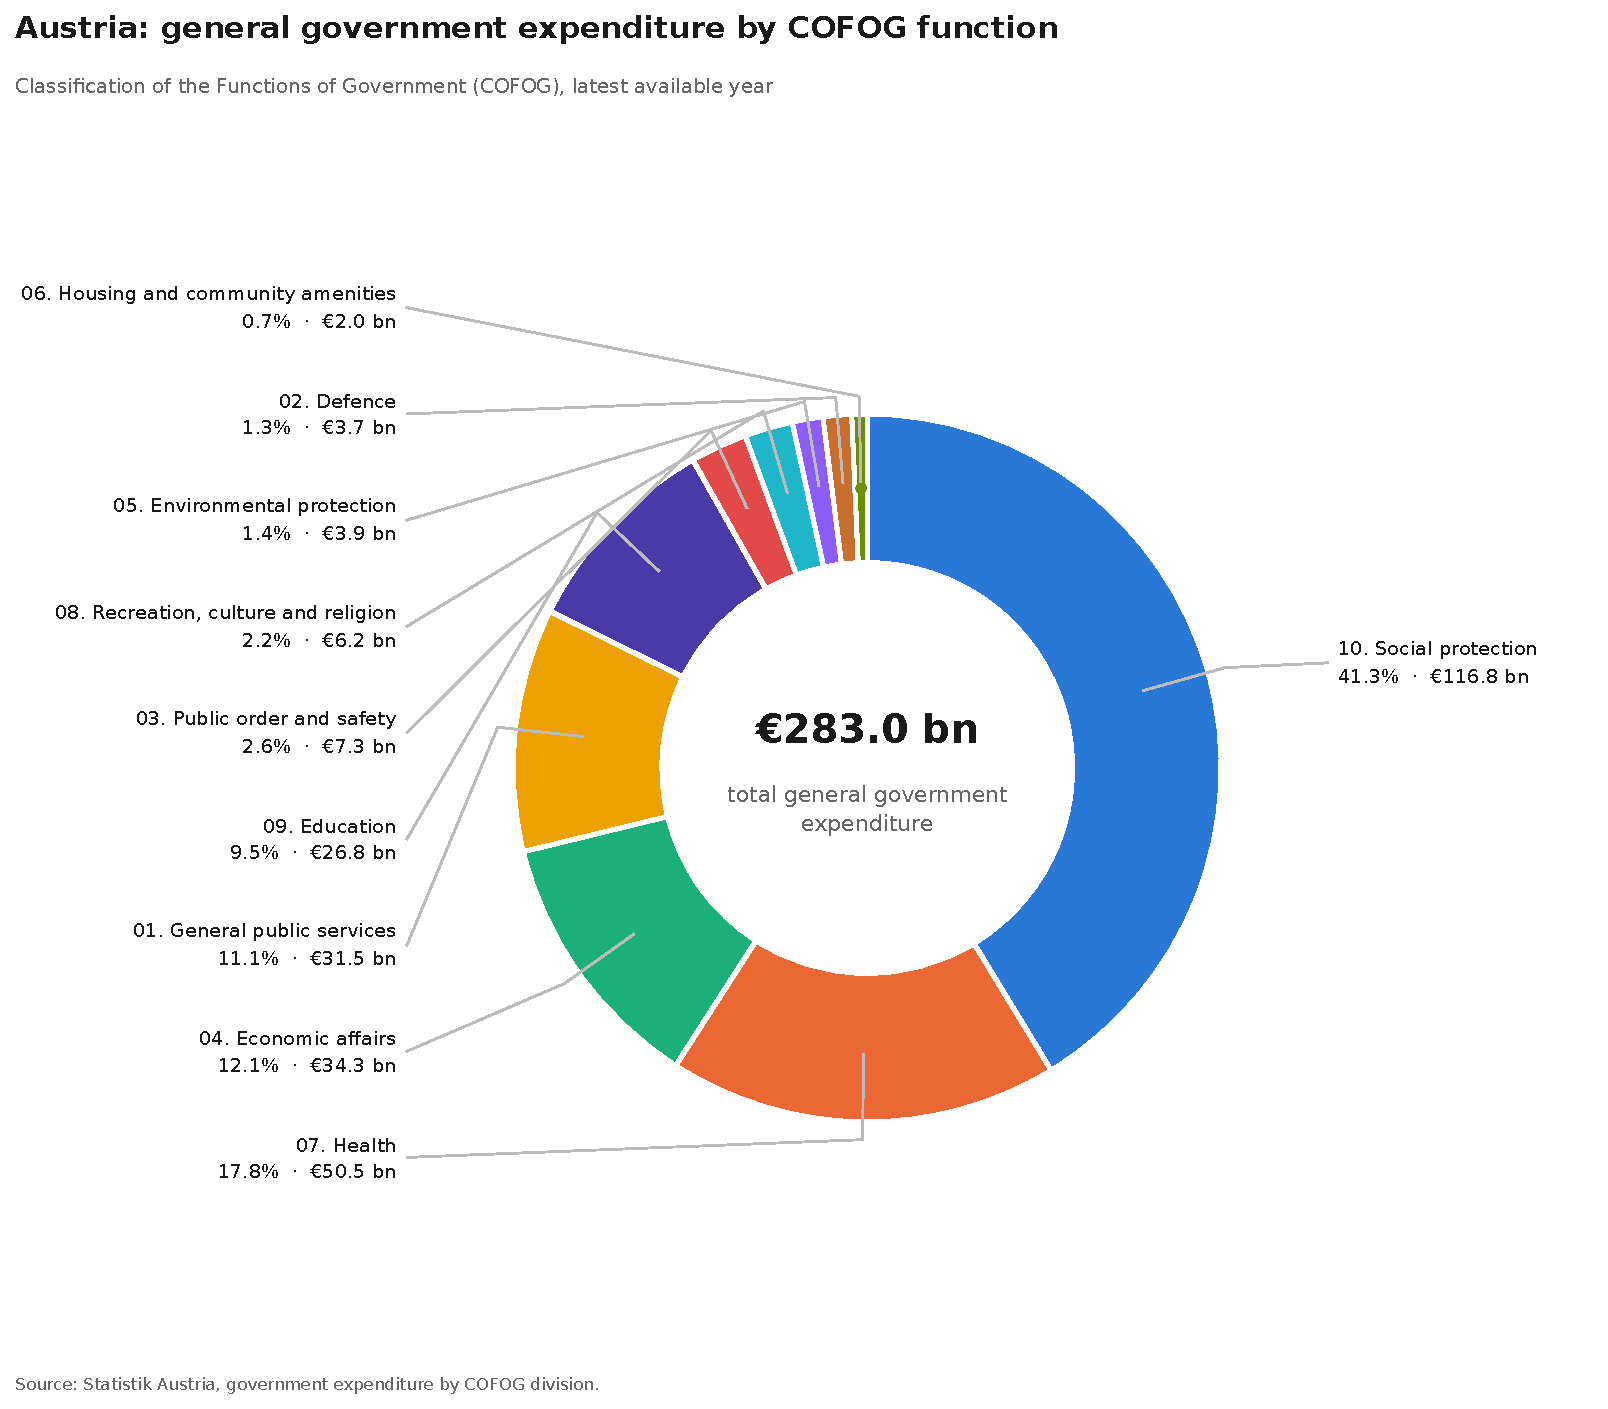
\includegraphics[width=0.7\linewidth]{austria_cofog_pie}
 \end{figure}
\end{frame}


\begin{frame}{Where Does the Revenue Come From?}
  Across many advanced economies, tax structures have shifted over recent decades --- away from taxing corporate profits, toward taxing labor income and consumption.
  \begin{block}{Discussion}
    What are the implications of shifting the tax burden from businesses toward workers' earnings?
  \end{block}
\end{frame}

\begin{frame}{Austria's Tax Mix: Heavy on Labor}
  \begin{itemize}
    \item VAT (\emph{Umsatzsteuer}): \(\approx\)26.2\% (2022)
    \item Wage tax (\emph{Lohnsteuer}): \(\approx\)58\% (2022)
    \item Capital tax (\emph{Kaptal}): \(\approx\)16\% (2022)

  \end{itemize}

    Austria taxes \textbf{labor} more heavily  than many other EU country.

  \srcnote{AK}
\end{frame}

\begin{frame}{Austria's Own Income-Distribution Data}
  \begin{itemize}
    \item Austria has its own ``Distributional National Accounts'' (DINA) research, in the tradition of Piketty--Saez--Zucman's work for the US and France.
    \item Jestl \& List (2020) construct such series for Austria, 2004--2016.

  \end{itemize}

\end{frame}

\begin{frame}{Pre-Tax national income per capita}
\begin{figure}
	\centering
	\includegraphics[width=0.7\linewidth]{"pretax income"}


\end{figure}
\end{frame}

\begin{frame}{Average annual real growth rates}

\begin{figure}
	\centering
	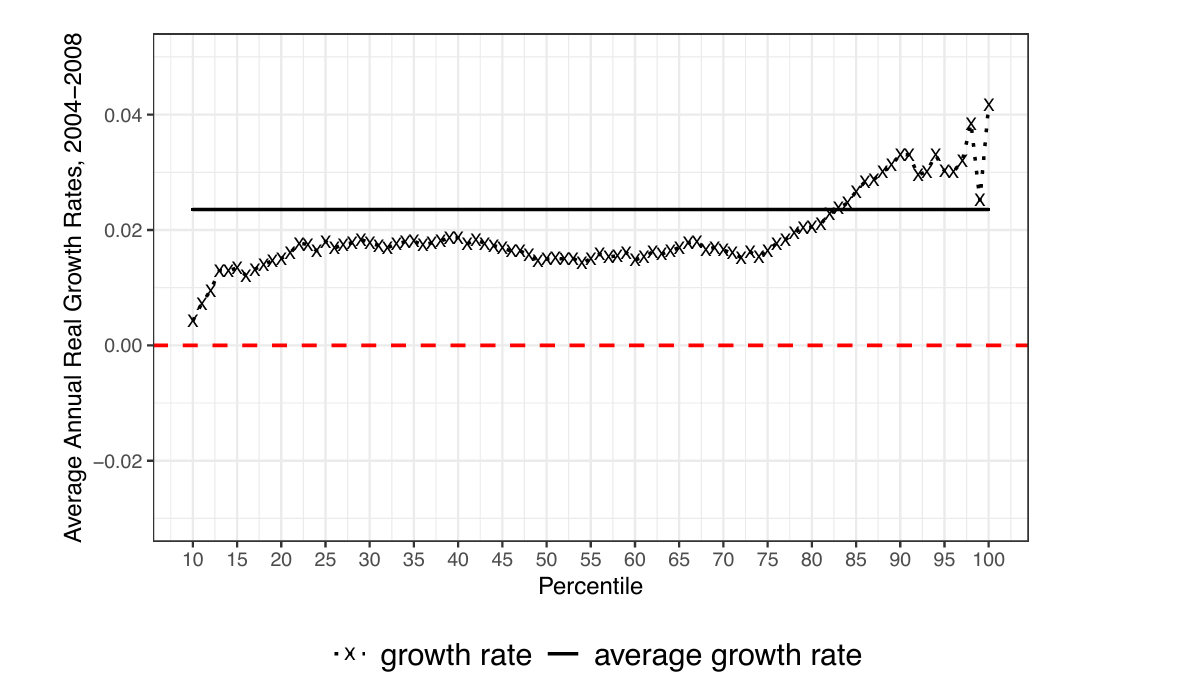
\includegraphics[width=0.5\linewidth]{growthrate_200408}
	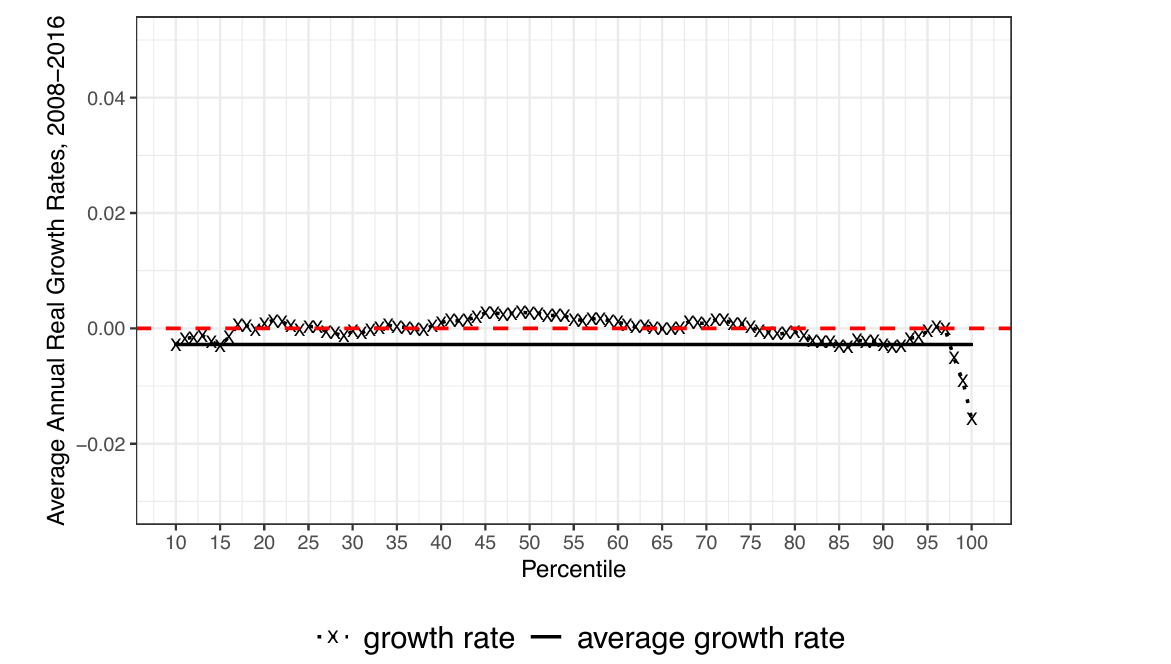
\includegraphics[width=0.5\linewidth]{growthrate_200816}
\end{figure}
\end{frame}



 \begin{frame}{Gini coefficient– pre-tax income and  post-tax income, 2004-2016}

 \begin{figure}
 	\centering
 	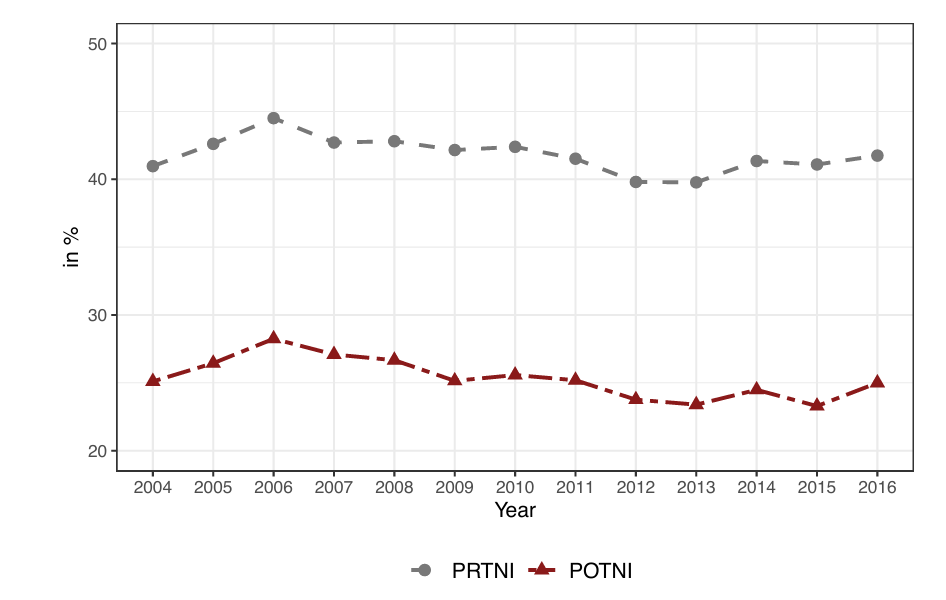
\includegraphics[width=0.7\linewidth]{pretaxposttax}

 \end{figure}
  \end{frame}

  \begin{frame}{Comparison with France and USA, top 10\%}
  \begin{figure}
	\centering
	\includegraphics[width=0.7\linewidth]{"country comparison"}
\end{figure}
  \end{frame}


\begin{frame}{Austria's Tax System, Top to Bottom}
  \begin{center}
  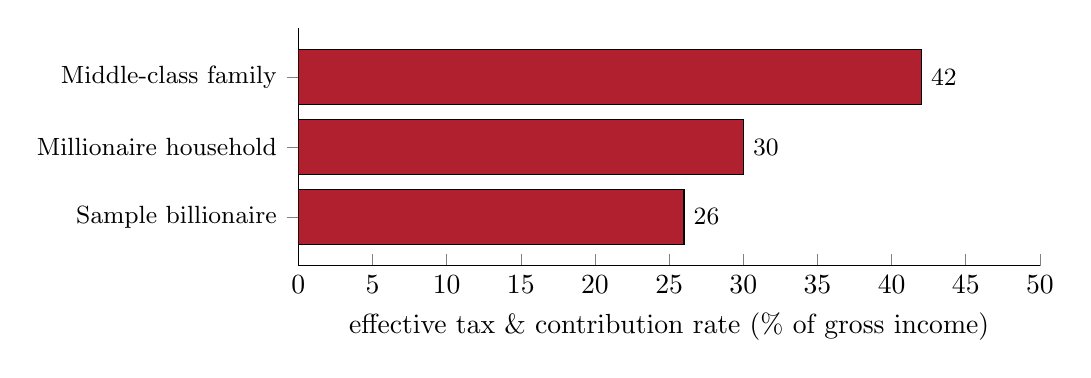
\begin{tikzpicture}
    \begin{axis}[
      xbar, bar width=0.7cm,
      width=11cm, height=4.6cm,
      xmin=0, xmax=50,
      symbolic y coords={Sample billionaire,Millionaire household,Middle-class family},
      ytick=data,
      y tick label style={font=\small},
      xlabel={effective tax \& contribution rate (\% of gross income)},
      nodes near coords,
      nodes near coords style={font=\small},
      enlarge y limits=0.35,
      axis lines*=left,
      ]
      \addplot[fill=wured] coordinates {
        (42,Middle-class family) (30,Millionaire household) (26,Sample billionaire)
      };
    \end{axis}
  \end{tikzpicture}
  \end{center}
   \small
  The statutory top income-tax rate is 55\%---but a billionaire's \emph{income} is mostly business profit and capital gains, taxed on different (lower, flatter) terms than wages.\\
  \srcnote{Momentum Institut, ``Problem Steuerstruktur: Arbeit hoch besteuert, Vermögen niedrig,'' Policy Brief 2022.01; ``Niedrigsteuerland für Superreiche.''}
\end{frame}











% =============================================================


\begin{frame}[standout]
  Thank you!\\
  \vspace{0.5em}
  \small Questions and discussion
\end{frame}

\end{document}
